\chapter{ZX Calculus}

\section{Generators}

\subsection{Z and X Spiders}

\subsection{Single Qubit Rotations}
An arbitrary rotation in the $X$ basis can be depicted by a single $X$ spider with phase $\alpha$.

\begin{figure}[H]
\centering
    \begin{minipage}{.3\textwidth}
      \centering
      \includegraphics[width=0.8\linewidth]{zx_calculus/z_rotation}
    \end{minipage}%
    \begin{minipage}{.3\textwidth}
      \centering
      \includegraphics[width=0.8\linewidth]{zx_calculus/x_rotation}
    \end{minipage}%
    \begin{minipage}{.3\textwidth}
      \centering
      \includegraphics[width=0.8\linewidth]{zx_calculus/hadamard}
    \end{minipage}
    \begin{minipage}{.3\textwidth}
      \centering
      \includegraphics[width=0.7\linewidth]{blochspheres/z_rotation}
    \end{minipage}
    \begin{minipage}{.3\textwidth}
      \centering
      \includegraphics[width=0.65\linewidth]{blochspheres/x_rotation}
    \end{minipage}
    \begin{minipage}{.3\textwidth}
      \centering
      \includegraphics[width=0.59\linewidth]{blochspheres/hadamard}
    \end{minipage}
    \caption{Bloch sphere representation.}
\end{figure}

